The main component of the CE architecture, illustrated in Figure~\ref{fig:ce-scheme}, is the 
128-channel FEMB, which itself consists of an analog motherboard and an attached COLDATA 
mezzanine card for processing the digital outputs.
Each APA is instrumented with 20 FEMBs, for a total of 2,560 channels per APA.
The FEMBs plug directly into the APA CR boards, making the connections from the U- and V-plane induction wires and 
X-plane collection wires to the charge amplifier circuits as short as possible.

\begin{dunefigure}
[The CE architecture. The basic unit is the 128-channel FEMB.]
{fig:ce-scheme}
{The CE architecture. The basic unit is the 128-channel FEMB.}
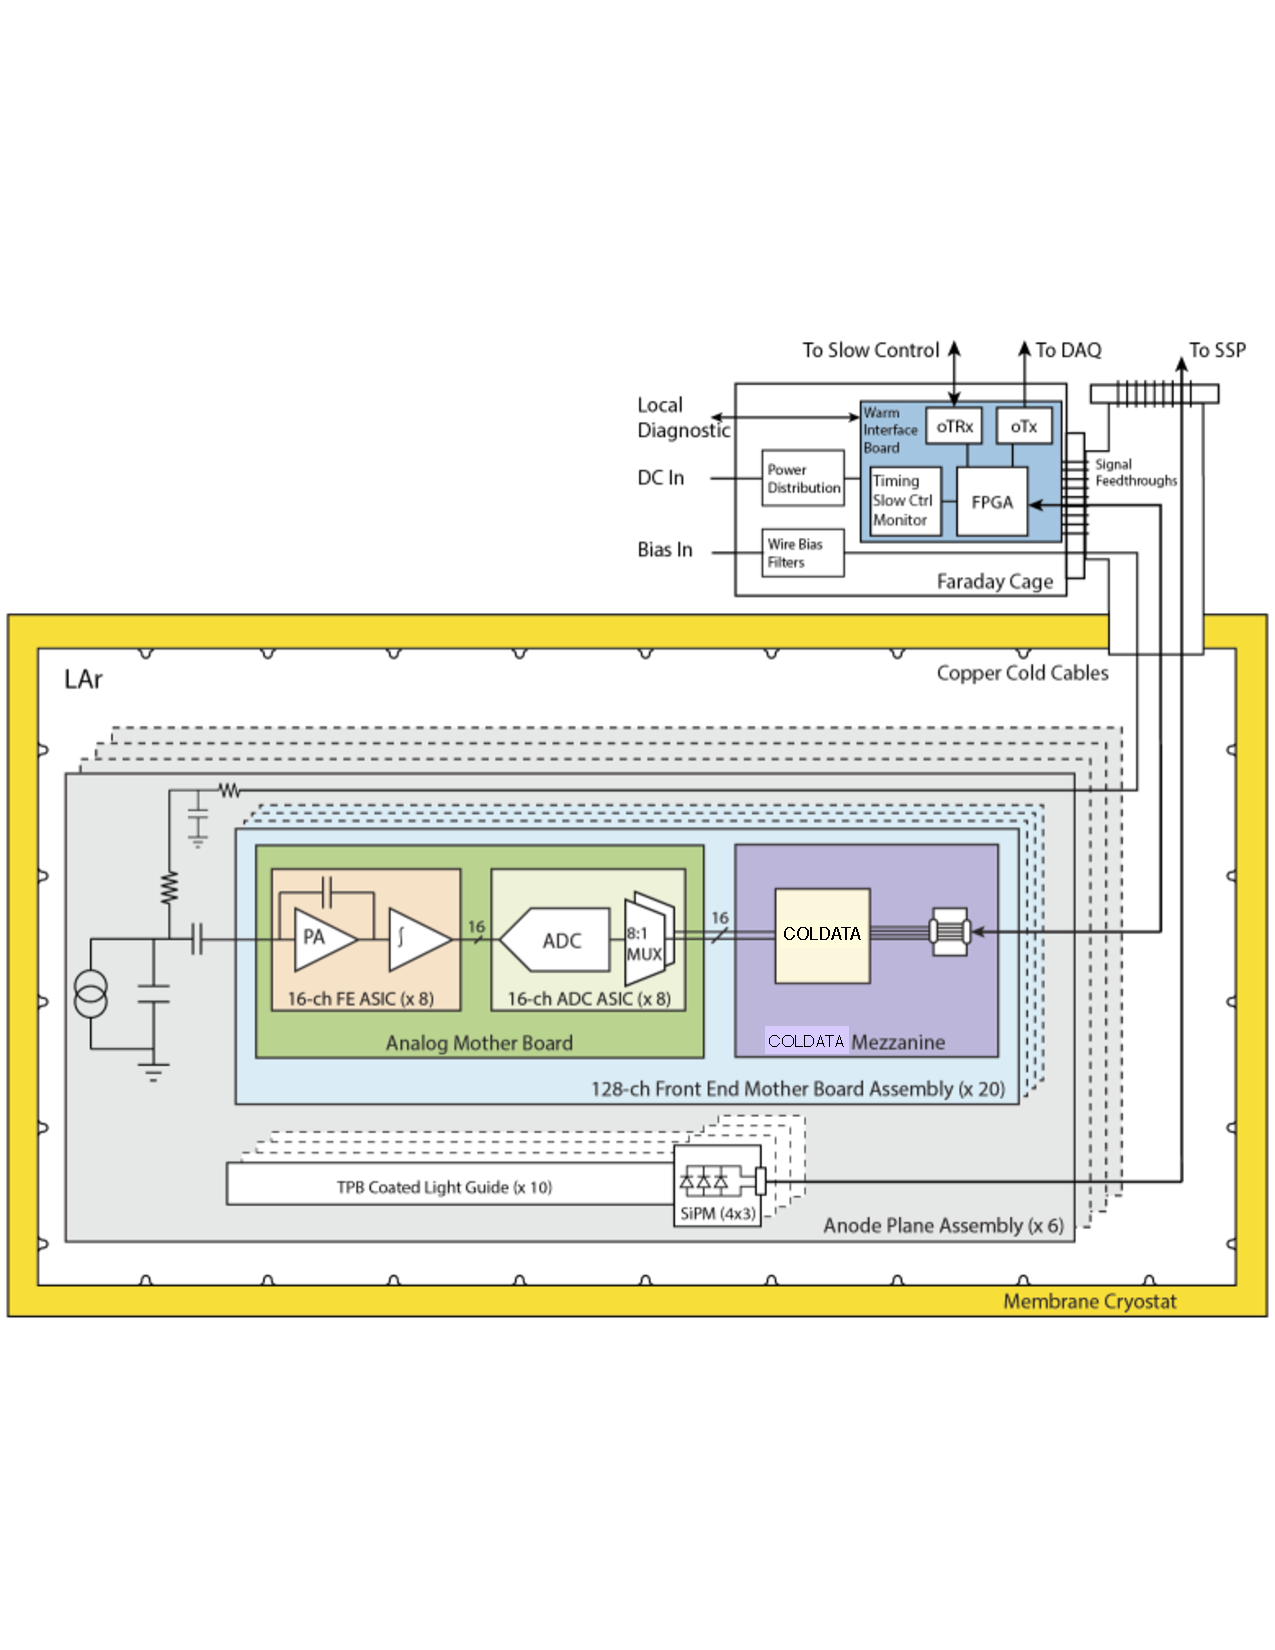
\includegraphics[width=0.9\linewidth]{tpcelec-schem_v2.pdf}
\end{dunefigure}
